\chapter{積分の離散近似}
    この部は文献\cite{digital-servo}に動機付けられて書いたものであり、その内容を再確認、深堀りしたもの、また派生して考えたことを記している。
    \section{Euler法}
        \subsection{背景}
            物理系をディジタル計算機で制御するにあたり、積分をEuler法で近似することがある。
            本節では正弦波をEuler法で近似的に積分した際の出力の窓関数付きFourier変換を導出し、高周波領域での位相変化、エイリアシングについて考察する。
        \subsection{導出}
            \newcommand{\xdd}{x_\text{dd}}
            $f_0>0$とし、連続時間の複素正弦波信号$u:t\in\realNumbers\mapsto\exp(i 2\pi f_0 t)$を考える。
            これを時刻$0$から$t\geq 0$まで積分した信号は$v(t) = \bigl(\exp(i 2\pi f_0 t)-1\bigr) / (i 2\pi f_0)$である。
            \ref{0次ホールドされた正弦波の周波数特性}と同様に、矩形窓を通した、周波数表示された$v$のFourier変換を考える(窓の幅をサンプリング周期の整数倍に限っても影響が少ないことの説明は\ref{0次ホールドされた正弦波の周波数特性}で述べられている)。
            $N\in\naturalNumbers$とし、窓の幅を$T=N\Ts$とする。
            $v$の窓付きFourier変換を窓の幅で規格化したものは次式である。
            但し計算は容易なので過程は省略した。
            \begin{align*}
                &\phantom{=} V(f) = \frac{1}{T} \integrate{0}{T}{v(t)\exp(-i 2\pi f t)}{}{t} \\
                &= \frac{1}{i 2\pi f_0 T} \left\{\frac{1}{i 2\pi (f-f_0)}\bigl[1 - \exp\bigl(-i 2\pi (f-f_0)T\bigr)\bigr] + \frac{1}{i 2\pi f}\bigl(\exp(-i 2\pi f T) - 1\bigr)\right\}
            \end{align*}
            次に、$u$の積分をサンプリング周期$\Ts>0$のEuler法で近似したものを考える。
            Euler法で積分した結果の離散時間信号を$\xdd:\integers\to\complexNumbers$とすると、これは漸化式$\xdd(n) = \xdd(n-1) + \Ts u\bigl((n-1)\Ts\bigr)$に従う。
            但し初期条件として$\xdd(0)=0$とする。
            この漸化式を解き、次式を得る。
            \[ \xdd(n) = \Ts\frac{1-\exp(i 2\pi f_0 n\Ts)}{1-\exp(i 2\pi f_0\Ts)} \]
            これを0次ホールドして得られる連続時間信号を$\xd(t) \coloneqq \xdd(\floor{t/\Ts}\Ts)$とする。
            先ほど$v$に対して行ったのと同様に窓付きFourier変換$\Xd$を計算すると、次式を得る。
            但し計算は容易なので過程の多くを省略した。
            \begin{align*}
                &\phantom{=} \Xd(f) = \frac{1}{T} \integrate{0}{T}{\xd(t)\exp(-i 2\pi f t)}{}{t} = \sum_{k=0}^{N-1} \frac{1}{T} \integrate{k\Ts}{(k+1)\Ts}{\xd(t)\exp(-i 2\pi f t)}{}{t} \\
                &= \frac{1}{i 2\pi f N}\times\frac{1-\exp(-i 2\pi f\Ts)}{1-\exp(i 2\pi f_0\Ts)} \left\{\frac{1-\exp(-i 2\pi f \Ts N)}{1-\exp(-i 2\pi f \Ts)} - \frac{1-\exp(-i 2\pi (f-f_0) \Ts N)}{1-\exp(-i 2\pi (f-f_0) \Ts)}\right\}
            \end{align*}
            $v$中の、周波数が$f_0$である成分の振幅と位相を調べる。
            $f\to f_0$の極限に関して次式が成り立つ。
            \[ \lim_{f\to f_0} V(f) = \frac{1}{i2\pi f_0}\left[1 + \frac{\exp(-i 2\pi f_0 T)-1}{i 2\pi f_0 T}\right] \]
            次に$\xd$中の、周波数が$f_0$である成分の振幅と位相を調べる。
            但し、$f_0\Ts < 1$と仮定する。
            次式が成り立つ。
            \[ \lim_{f\to f_0} \Xd(f) = \frac{1}{i 2\pi f_0 N}\times\frac{1-\exp(-i 2\pi f_0\Ts)}{1-\exp(i 2\pi f_0\Ts)}\left\{\frac{1-\exp(-i 2\pi f_0 \Ts N)}{1-\exp(-i 2\pi f_0 \Ts)} - N\right\} \]
            サンプリング周波数が十分高い、すなわち$f_0\Ts\ll 1$であるとき、次の近似式が成り立つ。
            \begin{align*}
                \lim_{f\to f_0} \Xd(f) &\approx \frac{1}{i 2\pi f_0 N}\times(-1)\left[\frac{1-\exp(-i 2\pi f_0 \Ts N)}{i 2\pi f_0 \Ts} - N\right] \\
                &= \frac{1}{i 2\pi f_0}\left[1 + \frac{\exp(-i 2\pi f_0 \Ts N)-1}{i 2\pi f_0 \Ts N}\right] = \frac{1}{i 2\pi f_0}\left[1 + \frac{\exp(-i 2\pi f_0 T)-1}{i 2\pi f_0 T}\right] \\
                &=  \lim_{f\to f_0} V(f)
            \end{align*}
        \subsection{数値例}
            今、$f_0=10,\;\Ts=10^{-2},\;N=200$とする。
            $f=f_0$に於ける$v$の振幅と位相の組は$(1/(20\pi),\;-\pi/2) \approx(1.59\times10^{-2},-1.57)$である。
            一方、$\xd$の振幅と位相の組はおよそ$(1.59\times10^{-2},-2.20)$である。
            \par
            次の図は$f_0$近傍でのエネルギー・スペクトラム密度$V,\Xd$を示したものである。
            \begin{figure}[H]
                \centering
                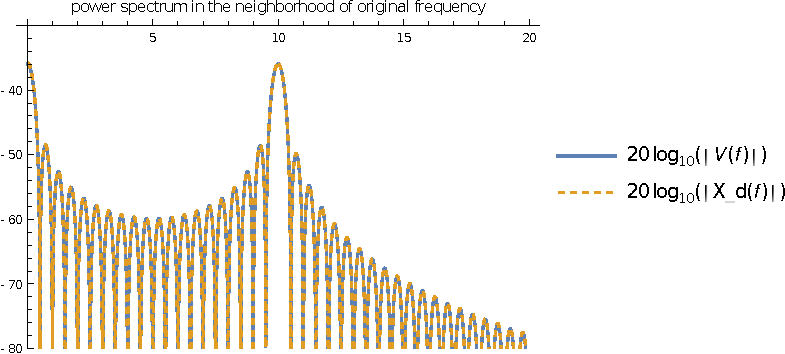
\includegraphics[keepaspectratio, scale=0.8]
                {\currfiledir/spectrum_in_the_neighborhood_of_original_frequency.pdf}
                \caption{元の周波数の近傍でのエネルギー・スペクトラム密度}
            \end{figure}
            低周波領域では絶対値が良く一致していることがわかる。
            \par
            次に高調波を見る。
            次の図はサンプリング周波数の3倍の範囲まで$V,\Xd$を示したものである。
            \begin{figure}[H]
                \centering
                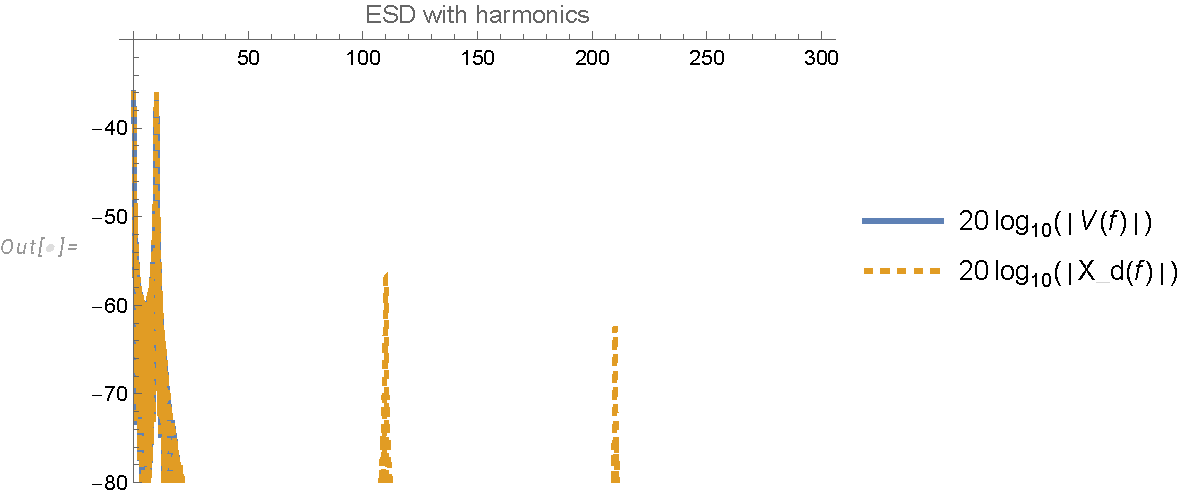
\includegraphics[keepaspectratio, scale=0.8]
                {\currfiledir/ESD_with_harmonics.pdf}
                \caption{高調波を含むエネルギー・スペクトラム密度}
            \end{figure}
            低周波の領域では$V,\Xd$が重なって判別できない。
            また、サンプリング周波数の整数倍の位置に高調波が生じていることが判る。
            \par
            この数値例を計算したMathematicaノートブックおよびMATLABスクリプトは下記のファイル名で保存されている。
            Gitリポジトリ内でファイル名検索すれば発見できるであろう。
            \begin{itemize}
                \item \href{\currfiledir/spectrum_of_integral-sine-wave_by_Euler-method.nb}{spectrum\_of\_integral\-sine-wave\_by\_Euler-method.nb}
                \item \href{\currfiledir/spectrum_of_integral_sine_wave_by_Euler_method.m}{spectrum\_of\_integral\_sine\_wave\_by\_Euler\_method.m}
            \end{itemize}
